\subsection{次数群为有序群的情形}

一个序结构（记作 \(\leqslant\) ）在写成加法形式的交换群 \(\Delta\) 上称为与群结构相容，如果对所有 \(\rho\in\Delta\) ，关系 \(\lambda\leqslant\mu\) 蕴含 \(\lambda+\rho\leqslant\mu+\rho\) 。带有这个序结构的群 \(\Delta\) 称为有序群。我们将在 VI, §1 中详细研究这些群；这里只指出，在这样的群中，关系 \(\lambda>0\) 蕴含 \(\lambda+\mu>\mu\) （对所有 \(\mu\) ），因为它按定义蕴含 \(\lambda+\mu\geqslant\mu\) ，而关系 \(\xi+\mu=\mu\) 等价于 \(\xi=0\) 。

设 \(\Delta\) 是一个有序交换群，A 是一个类型为 \(\Delta\) 的分次环， \((\mathbf{A}_{\lambda})\) 是它的分次，并设关系 \(\mathbf{A}_{\lambda} \neq \{0\}\) 蕴含 \(\lambda \geqslant 0\) ；则由定义可知 \(\mathfrak{I}_0 = \sum_{\lambda > 0} \mathbf{A}_{\lambda}\) 是 A 的一个分次双边理想（据上述注记）。

命题6. 设 \(\Delta\) 是一个有序交换群，A 是一个类型为 \(\Delta\) 的分次环， \((\mathbf{A}_{\lambda})\) 是它的分次，M 是一个类型为 \(\Delta\) 的分次 A-模， \((\mathbf{M}_{\lambda})\) 是它的分次。设关系 \(\mathbf{A}_{\lambda} \neq \{0\}\) 蕴含 \(\lambda \geqslant 0\) ，且存在 \(\lambda_0\) 使得 \(\mathbf{M}_{\lambda_0} \neq \{0\}\) 而 \(\mathbf{M}_{\lambda} = \{0\}\) （对 \(\lambda < \lambda_0\) ）。则若 \(\Im_0 = \sum_{\lambda > 0} \mathbf{A}_{\lambda}\) ，就有 \(\Im_0 \mathbf{M} \neq \mathbf{M}\) 。

设 \(x\) 是 \(\mathbf{M}_{\lambda_0}\) 的一个非零元素；设 \(x \in \mathfrak{I}_0\mathbf{M}\) 。则 \(x = \sum_{i} a_i x_i\) ，其中诸 \(a_i\) 是齐次元素 \(\neq 0\) （ \(\mathfrak{I}_0\) 中的），诸 \(x_i\) 是齐次元素 \(\neq 0\) （ \(\mathbf{M}\) 中的），且 \(\deg(x) = \deg(a_i) + \deg(x_i)\) （对所有 \(i\) ）（第 2 号）。但是，由于 \(\deg(a_i) > 0\) ，有 \(\lambda_0 = \deg(a_i) + \deg(x_i) > \deg(x_i)\) ，这与假设矛盾。

推论1. 在命题 6 对 \(\Delta\) 与 A 的假设下，若 \(M\) 是一个使 \(\mathfrak{S}_0\mathbf{M} = \mathbf{M}\) 的有限生成分次 A-模，则 \(\mathbf{M} = \{0\}\) 。

设 \(M \neq \{0\}\) 。令 \(\lambda_{0}\) 为 M 的一个由齐次元素 \(\neq0\) 组成的有限生成系的次数集合中的极小元素；那么命题 6 的假设将被满足，这就导出矛盾。

推论2. 在命题 6 对 \(\Delta\) 与 A 的假设下，设 M 是一个有限生成分次 A-模，N 是 M 的一个分次子模，使得 \(N + I_{0}M = M\) ；则 N = M。

M/N 是一个有限生成分次 A-模，且该假设蕴含 \(\mathfrak{S}_{0}(\mathbf{M}/\mathbf{N}) = \mathbf{M}/\mathbf{N}\) ；因此 M/N = 0。

推论3. 在命题 6 对 \(\Delta\) 与 A 的假设下，令 \(u: \mathbf{M} \to \mathbf{N}\) 是分次右 A-模的一个分次同态，其中假设 N 是有限生成的。若同态

\[
u \otimes 1: \mathbf {M} \otimes_ {\mathbf {A}} (\mathbf {A} / \mathfrak {I} _ {0}) \rightarrow \mathbf {N} \otimes_ {\mathbf {A}} (\mathbf {A} / \mathfrak {I} _ {0})
\]

是满射，则 u 是满射。

\(u(\mathbf{M})\) 是 \(\mathbf{N}\) 的一个分次子模，而 \((\mathbf{A} / \mathfrak{I}_0)\) -模

\[
(\mathbf {N} / u (\mathbf {M})) \otimes_ {\mathbf {A}} (\mathbf {A} / \mathfrak {I} _ {0})
\]

同构于 \((\mathbf{N} \otimes_{\mathbf{A}} (\mathbf{A} / \mathfrak{I}_0)) / \mathrm{Im}(u \otimes 1)\) （§3, 第 6 号, 命题 6）。因此该假设蕴含 \((\mathbf{N} / u(\mathbf{M})) \otimes_{\mathbf{A}} (\mathbf{A} / \mathfrak{I}_0) = 0\) ，从而由推论 1 得 \(\mathbf{N} = u(\mathbf{M})\) 。

注. 由推论 1 的证明可知，推论 1 和推论 2（相应地，推论 3）在下述假设下仍然成立：不假设 M（相应地，N）是有限生成的，而是假设存在一个子集 \(\Delta^{+}\) （ \(\Delta\) 的），满足以下条件：

\begin{enumerate}
\def\labelenumi{(\arabic{enumi})}
\item
  对 \(\lambda \notin \Delta^{+}\) ，有 \(\mathbf{M}_{\lambda} = \{0\}\) （相应地， \(\mathbf{N}_{\lambda} = \{0\}\) ）；
\item
  \(\Delta^{+}\) 的每个非空子集有一个最小元素。
\end{enumerate}

当 \(\Delta = Z\) 且 M（相应地，N）是具有正次数的分次模时，就是这种情形。

命题7. 设 \(\Delta = \mathbf{Z}\) 。在命题 6 对 A 和 M 的假设下，考虑分次 \(\mathbf{A}_0\) -模 \(\mathbf{N} = \mathbf{M} / \Im_0\mathbf{M}\) ，并设以下条件成立：

\begin{enumerate}
\def\labelenumi{(\roman{enumi})}
\item
  每个 \(\mathbf{N}_{\lambda}\) （视为 \(\mathbf{A}_0\) -模）都具有一组基 \((y_{\iota \lambda})_{\iota \in I_{\lambda}}\) ；
\item
  典范同态 \(\mathfrak{S}_0\otimes_{\mathbf{A}}\mathbf{M}\to \mathbf{M}\) 是单射。
\end{enumerate}

那么 \(\mathbf{M}\) 是一个分次自由 A-模（第 2 号，注 3），并且确切地说，若 \(x_{\iota \lambda}\) 是 \(\mathbf{M}_{\lambda}\) 的一个元素，它在 \(\mathbf{N}_{\lambda}\) 中的像是 \(y_{\iota \lambda}\) ，则族 \((x_{\iota \lambda})_{(\iota ,\lambda)\in \mathbf{I}}\) （其中 \(\mathbf{I}\) 是诸 \(\mathbf{I}_{\lambda}\) 之和的集合）是 \(\mathbf{M}\) 的一个基。

我们知道（第 2 号，注 3）存在一个分次自由 A-模 L（其分次为 \((\mathbf{L}_{\lambda})\) ）以及一个次数为 0 的满同态 \(p: \mathbf{L} \to \mathbf{M}\) ，使得 \(p(e_{t\lambda}) = x_{t\lambda}\) 对所有 \((t, \lambda) \in \mathbf{I} ((e_{t\lambda})_{(t,\lambda) \in \mathbf{I}}\) 是由齐次元素 \(e_{t\lambda} \in \mathbf{L}_{\lambda}\) 组成的 L 的一个基。由上述注可知 \(p\) 是满射。考虑分次 A-模 \(\mathbf{R} = \operatorname{Ker}(p)\) ，并注意按定义有 \(\mathbf{R}_{\lambda} = \{0\}\) （对 \(\lambda < \lambda_0\) ）；我们要证明 \(\mathbf{R} = \{0\}\) ，而由命题 6，只需证明 \(\mathfrak{S}_0\mathbf{R} = \mathbf{R}\) 。考虑交换图（§3, 第 6 号, 命题 5）

\pandocbounded{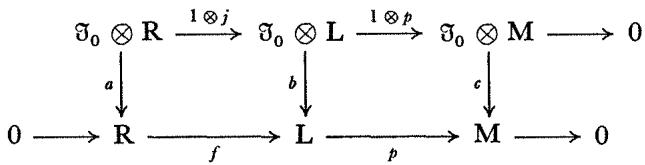
\includegraphics[keepaspectratio]{images/part003_24c814e1.jpg}}

其中 \(j\) 是典范单射， \(a, b, c\) 由典范单射 \(\mathfrak{I}_0 \to \mathbf{A}\) 导出（ \(\S 3\) , 第 4 号, 命题 4）；要证明的是 \(a\) 为满射。注意，由于 \(\mathbf{L}\) 是自由的， \(b\) 是单射的（ \(\S 3\) , 第 7 号, 命题 7 的推论 6），且 \(c\) 按假设是单射的。令 \(t\) 是 \(\mathbf{R}\) 的一个元素， \(t\) 是它在 \(\mathbf{R} / \mathfrak{I}_0\mathbf{R}\) 中的类；则有一个正合序列（ \(\S 3\) , 第 6 号, 命题 5 及命题 6 的推论 2）

\[
\mathrm{R} / \mathfrak {I} _ {0} \mathrm{R} \xrightarrow {\jmath} \mathrm{L} / \mathfrak {I} _ {0} \mathrm{L} \xrightarrow {\bar {p}} \mathrm{M} / \mathfrak {I} _ {0} \mathrm{M} \longrightarrow 0
\]

其中 \(j\) 和 \(\bar{p}\) 是 \(j\) 与 \(p\) 过渡到商时导出的，而 \(\bar{p}\) 按假设是双射；于是 \(\bar{j}(t) = 0\) ，换言之 \(j(t) \in \mathfrak{I}_0\mathbf{L}\) 。则存在一个元素 \(z \in \mathfrak{I}_0 \otimes \mathbf{L}\) 使得 \(j(t) = b(z)\) ；由于 \(p(b(z)) = 0\) ，有 \(c((1 \otimes p)(z)) = 0\) ，又由于 \(c\) 是单射，有 \((1 \otimes p)(z) = 0\) 。换言之， \(z\) 是某个元素 \(t' \in \mathfrak{I}_0 \otimes \mathbf{R}\) 在 \(1 \otimes j\) 下的像，于是 \(j(a(t')) = b(z) = j(t)\) ；由于 \(j\) 是单射，这就蕴含 \(t = a(t')\) 。

我们将在后文（交换代数, II, §3, 第 2 号, 命题 5）中说明如何把这命题推广到非分次模。

引理1. 交换群 \(\Delta\) 使得在 \(\Delta\) 上存在一个与 \(\Delta\) 的群结构相容的全序，其必要且充分的条件是 \(\Delta\) 无挠。

若在 \(\Delta\) 上存在这样一个序结构，且若 \(\lambda > 0\) ，则 \(\lambda + \mu > 0\) （对所有 \(\mu \geqslant 0\) ），特别地，对整数 \(n > 0\) 作归纳得 \(n.\lambda > 0\) ，这就证明 \(\Delta\) 是无挠的（因为每个元素 \(\neq 0\) （ \(\Delta\) 中的）或者 \(>0\) 或者 \(< 0\) ）。反之，若 \(\Delta\) 是无挠的，则 \(\Delta\) 是一个向量 \(\mathbf{Z}\) -空间的子 \(\mathbf{Q}\) -模（ \(\S 7\) , 第 10 号, 命题 26 的推论 1），可设它具有形式 \(\mathbf{Q}^{(I)}\) ；若给 I 一个良序（集合论, III, \(\S 2\) , 第 3 号, 定理 1），并给 \(\mathbf{Q}\) 其通常的序，则集合 \(\mathbf{Q}^{(I)}\) 赋予字典序是全序的（集合论, III, \(\S 2\) , 第 6 号）；立即看出这个序与 \(\mathbf{Q}^{(I)}\) 的加法群结构相容。

命题8. 设 \(\Delta\) 是一个无挠交换群，A 是一个类型为 \(\Delta\) 的分次环。若 A 中两个齐次元素 \(\neq 0\) 的乘积 \(\neq 0\) ，则环 A 没有零因子。

设 \(\Delta\) 被赋予与其群结构相容的全序（引理

\begin{enumerate}
\def\labelenumi{\arabic{enumi})}
\tightlist
\item
  ，并设 \(x = \sum_{\lambda \in \Delta} x_{\lambda}, y = \sum_{\lambda \in \Delta} y_{\lambda}\) 是 A 的两个非零元素（ \(x_{\lambda}\) 和 \(y_{\lambda}\) 是次数为 \(\lambda\) 的齐次元素，对所有 \(\lambda \in \Delta\) ）；设 \(\alpha\) （相应地， \(\beta\) ）是元素 \(\lambda \in \Delta\) （使 \(x_{\lambda} \neq 0\) （相应地， \(y_{\lambda} \neq 0\) ）者）中最大的；立即看出，若 \(\lambda \neq \alpha\) 或 \(\mu \neq \beta\) ，则或者 \(x_{\lambda}y_{\mu} = 0\) 或者 \(\deg(x_{\lambda}y_{\mu}) < \alpha + \beta\) ；因此 \(xy\) 的次数为 \(\alpha + \beta\) 的齐次分量是 \(x_{\alpha}y_{\beta}\) ，它按假设非零；从而 \(xy \neq 0\) 。
\end{enumerate}

